\section{Braille}

\frame{
\frametitle{\secname}

\begin{figure}
\centering
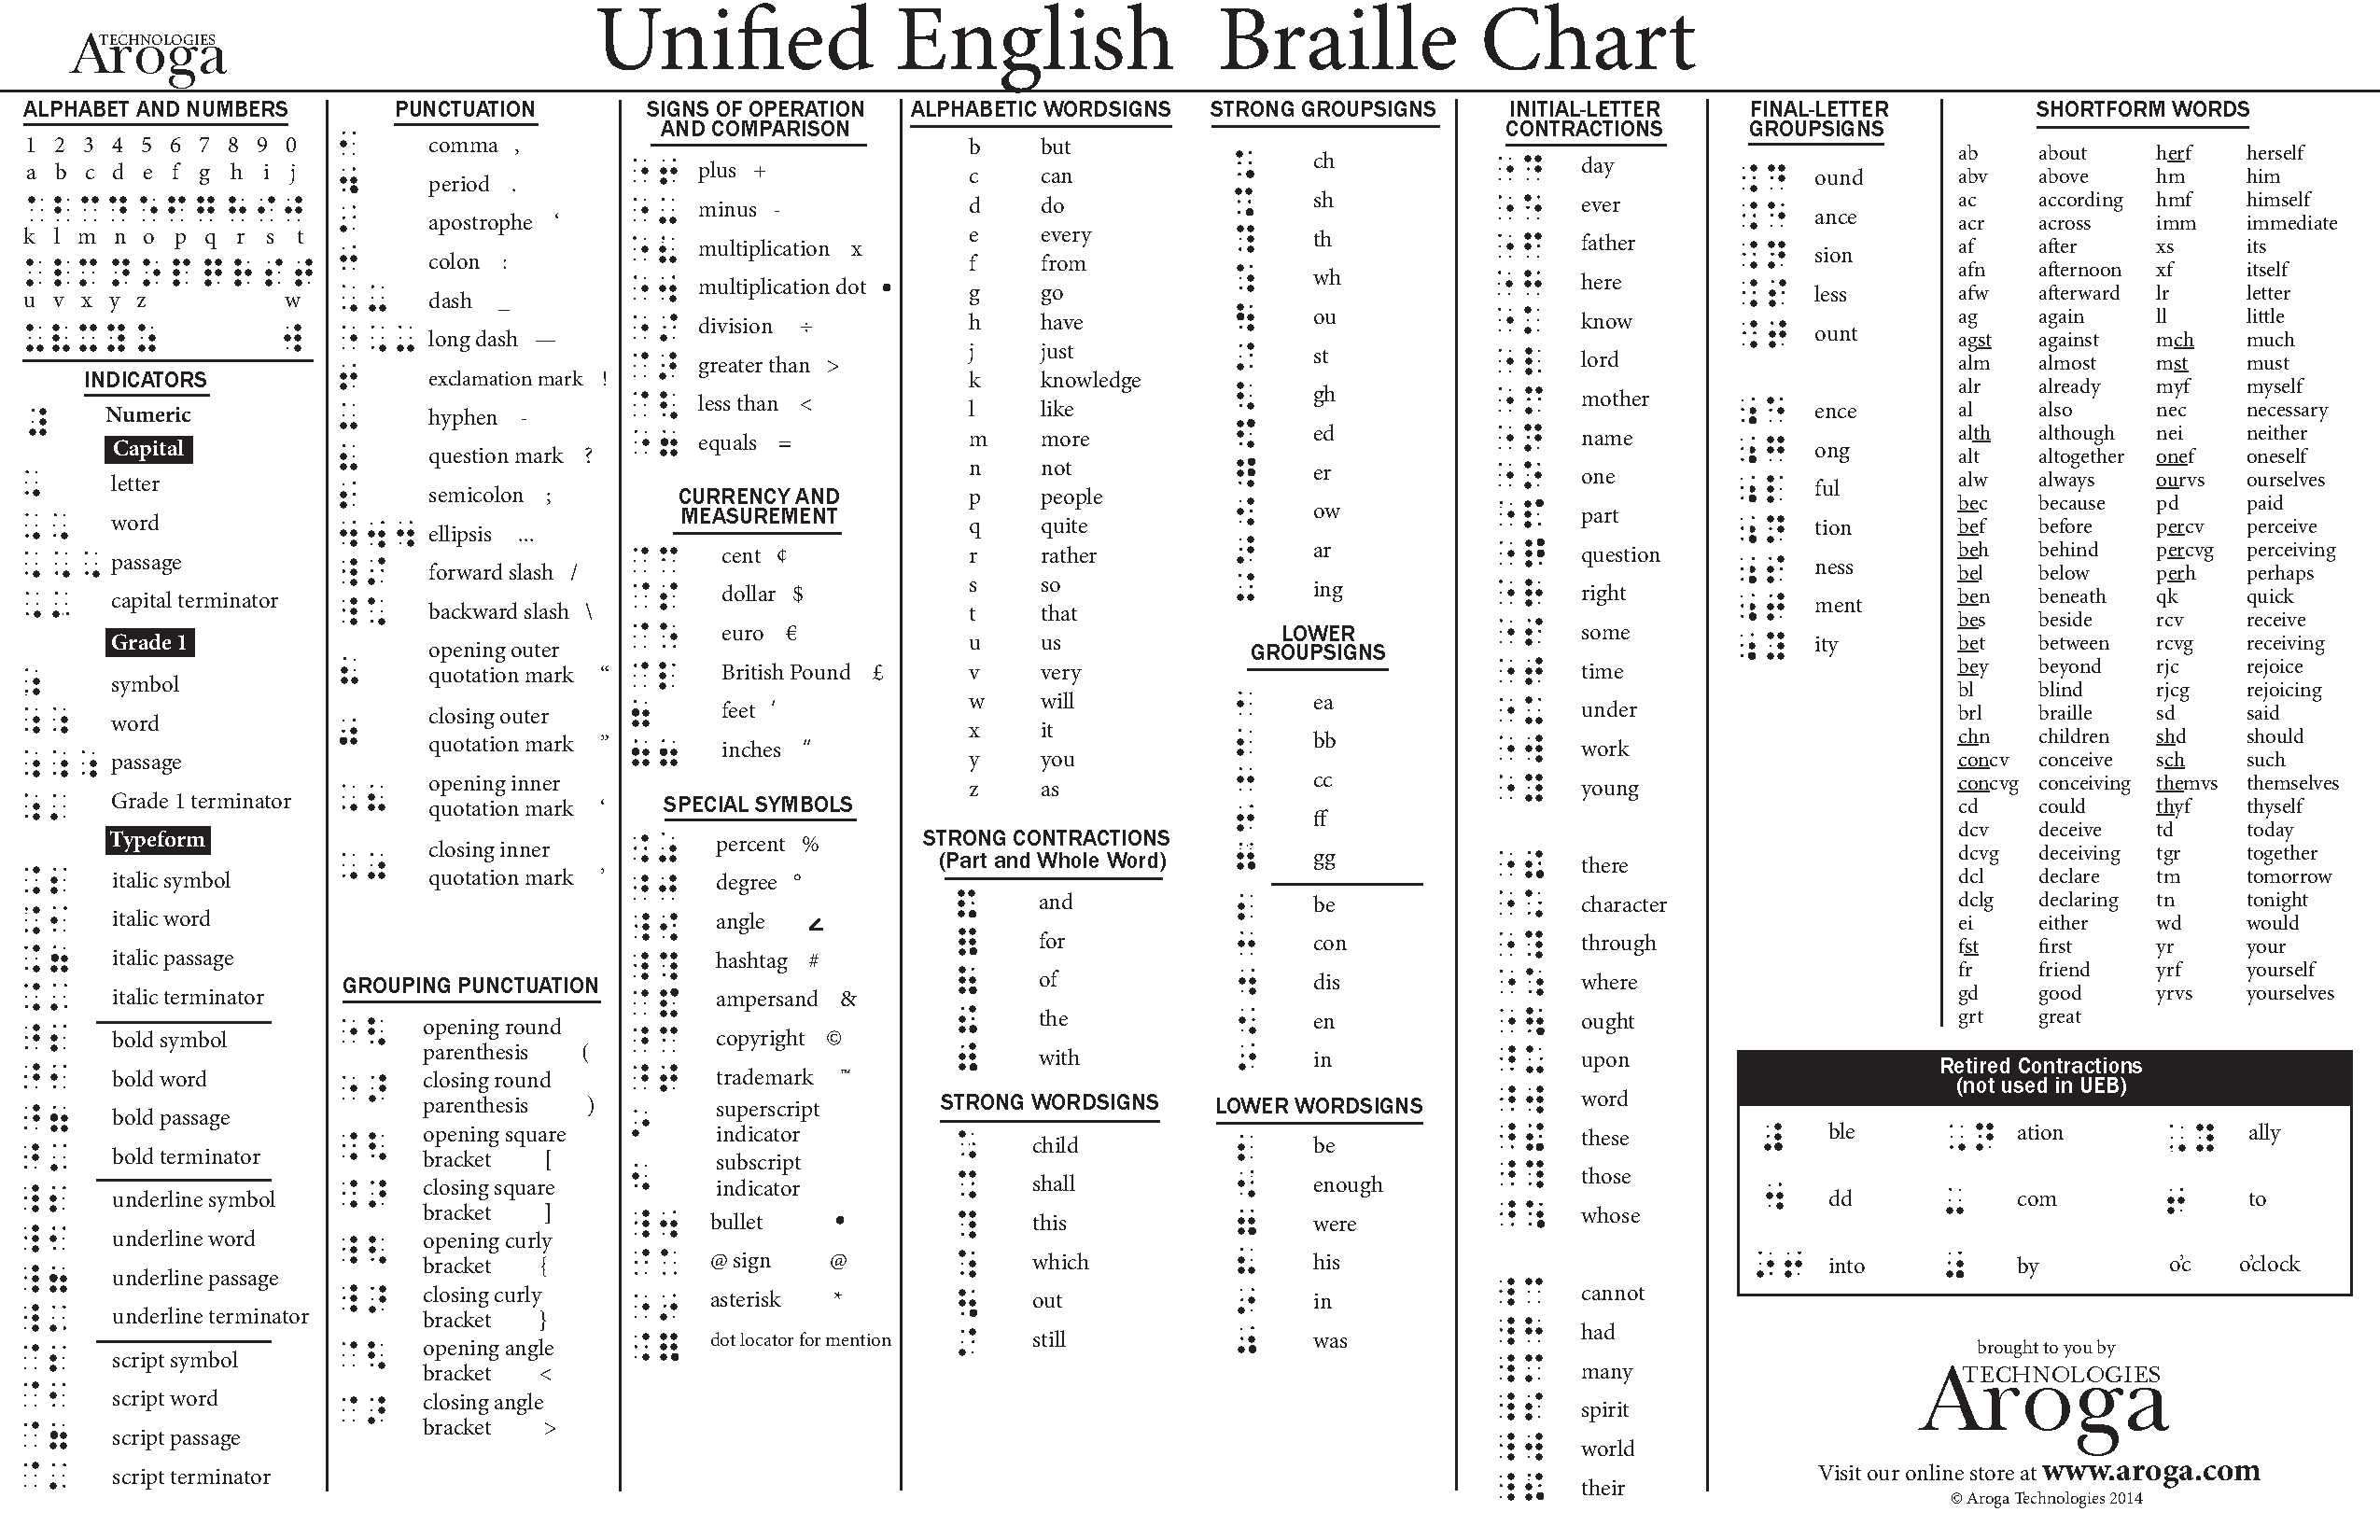
\includegraphics[width=0.65\textwidth]{slides/braille/ueb_braille_chart.pdf}
\end{figure}

}

\frame{
\frametitle{\secname}

\begin{columns}
\column{0.4\textwidth}
\begin{figure}
\centering
\brailleputtinydotstrue
\setlength{\tabcolsep}{0em}
\begin{tabular}{cccccccccc}
\multicolumn{10}{c}{\uppercase{Alphabet and numbers}} \\
\hline
1 & 2 & 3 & 4 & 5 & 6 & 7 & 8 & 9 & 0 \\
a & b & c & d & e & f & g & h & i & j \\
\braille{a} & \braille{b} & \braille{c} & \braille{d} & \braille{e} & \braille{f} & \braille{g} & \braille{h} & \braille{i} & \braille{j} \\

k & l & m & n & \alert<3->{o} & p & q & r & s & t \\
\braille{k} & \braille{l} & \braille{m} & \braille{n} & \alert<3->{\braille{o}} & \braille{p} & \braille{q} & \braille{r} & \braille{s} & \braille{t} \\

u & v & x & y & z &   &   &   &   & w \\
\braille{u} & \braille{v} & \braille{x} & \braille{y} & \braille{z}  &   &   &   &   & \braille{w}
\end{tabular}
\end{figure}

\column{0.4\textwidth}
\visible<2->{
\begin{figure}
\centering
\brailleputtinydotstrue
\setlength{\tabcolsep}{0em}
\begin{tabular}{rlrl}
\multicolumn{4}{c}{\uppercase{Strong groupsigns}} \\
\hline
\quad\braille{{ch}}\quad\null & \quad ch & \quad\braille{{gh}}\quad\null & \quad gh\\
\quad\braille{{sh}}\quad\null & \quad sh & \quad\braille{{ed}}\quad\null & \quad ed\\
\quad\braille{{th}}\quad\null & \quad th & \quad\braille{{er}}\quad\null & \quad er\\
\quad\braille{{wh}}\quad\null & \quad wh & \quad\alert<3->{\braille{{ow}}}\quad\null & \quad \alert<3->{ow}\\
\quad\braille{{ou}}\quad\null & \quad ou & \quad\braille{{ar}}\quad\null & \quad ar\\
\quad\braille{{st}}\quad\null & \quad st & \quad\braille{{ing}}\quad\null & \quad ing
\end{tabular}
\end{figure}
}

\column{0.2\textwidth}
\visible<3->{
\alert{``owo" is \braille{{ow}o}}
}

\end{columns}

}